 Couchbase Server is designed to access real-time operational data. It is a NoSQL database that serves both as key-value and document-oriented database. As a key-value store, it is able to store any type of data including  strings, numbers and binary data and the data is treated as an opaque Binary Large Object(BLOB). When used as document store, data is stored in a valid JSON format. The data is stored in logical unit called buckets. These buckets are isolated to each other and have their own RAM quota and replica settings. Buckets can be compared with \texttt{database} of MongoDB or any other RDBMS. Couchbase recommends few number of buckets in a single cluster. 
 \todo{write about raplica settings and ram quota}
 
 A bucket can contain any type of data, but data other than JSON, can only be retrieved by its key. Therefore, before fetching, it is important to check metadata that is stored in a single document. Each document is stored independently and there is no notion of grouping documents like collections in MongoDB or tables in other RDBMS. An user-defined type attribute can be created to differentiate the various documents stored in the bucket and  create indexes on them.  For example, \textit{user} and \textit{post} are two collections of MongoDB. The documents of these two collections can be represented in Couchbase by adding a new field \textit{documentType}  in each document with value \textit{user} and \textit{post} respectively.  

\paragraph{Metadata}\label{cb-metadata}
%may be we can remove it.
For every value stored in a bucket, Couchbase generates following meta information that is associated with a document~\cite[p. 26]{cb/ostrovsky2014pro}. 
\begin{itemize}
	\item{Expiration time:}
		The Time to Live(TTL) also named as expiration time is the life time of a document. The default value of TTL is 0 that indicates document will never expire and also can be set as Unix epoch time after which document is removed.
	\item{Check-and-Set(CAS):}
		The CAS value is 64-bit integer that is updated by the server when associated item is modified. The document is updated only  if unique identifier matches the identifier of the document. CAS is used to manage concurrency when multiple client attempts to update the same document simultaneously. 
	\item{Flags:} 
Flags are SDK-specific parameter that are used to identify the format and the type of data objects being stored.
\item{Type:}
 \textit{type} is the type of a document either \textit{json} or Base64 encoded string.
 \item{Document Key:}
 Every value in Couchbase is saved with unique identifier called document key. Unlike MongoDB, in Couchbase the key should be manually generated. The key length should be with in 250 characters.
\end{itemize}	

%In case of XMark data each \texttt{id} attributes of  \texttt{item}, \texttt{person}, \texttt{open\_auction}, \texttt{category} represent as key. In case of  \texttt{closed\_auction} and  \texttt{edge} key can be manually generated. 
\begin{figure}[h]
	\centering
	\subfloat[Views in Document Design]{
		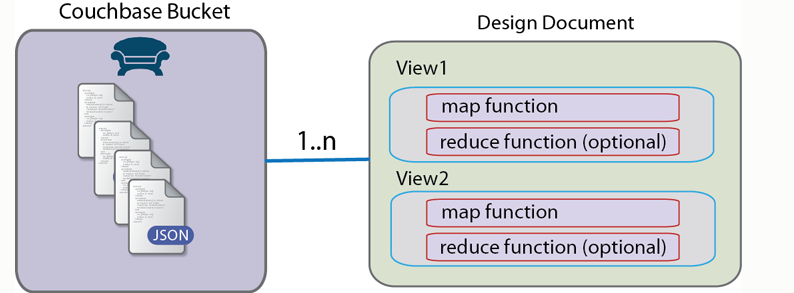
\includegraphics[width=0.4\textwidth]{img/cb/Small_view_elements}
		\label{fig:cb-views-design}
	}
	\centering
	\subfloat[View's Workflow]{
		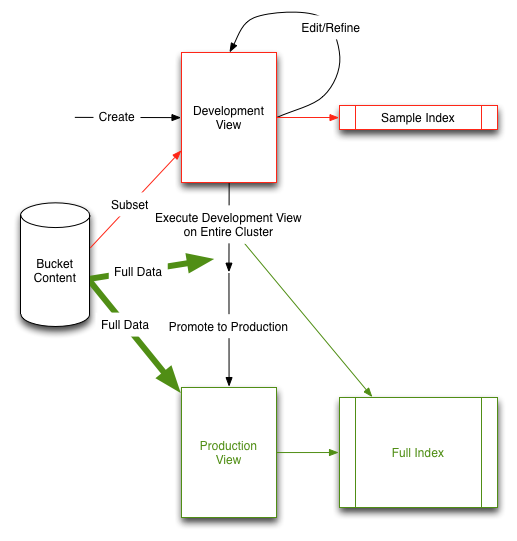
\includegraphics[width=0.4\textwidth]{img/cb/view-types-workflow}
		\label{fig:cb-views-workflow}
	}
	\caption{Couchbase Server's Document Design ~\citep{couchbasedocs}}
	\label{fig:cb-views-document-design}	
\end{figure}

\paragraph{Bucket and vBucket}
 Data bucket used by the Couchbase is a logical container of information that provides a logical grouping of physical resources within a cluster~\citep{lichtenberg2013nosql}. Documents in Couchbase do not have fixed structure. Each bucket is split into 1024 logical partitions called vBuckets. A vBucket is treated as a owner of subset of keys as shown in Figure~\ref{fig:cb-vbucket}.  
%%why we need vbucket

\begin{figure}[h]
	\centering
	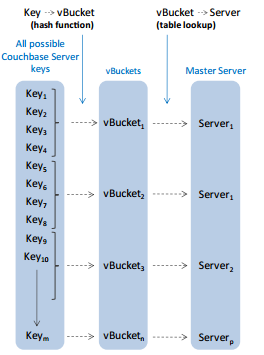
\includegraphics[width=0.4\textwidth]{img/vbucket2}
	\caption{ Couchbase Key, Bucket and   vBucket ~\cite{couchbasedocs}}
	\label{fig:cb-vbucket}
\end{figure}
%where is reference of images

\subsubsection{Data Model}%repeat check once
A document is a basic unit of data manipulation in Couchbase. All the documents are stored in JSON format without a predefined schema.

\subsubsection{Querying and Indexing}
Query in Couchbase has to be done against pre-materialize views. The goal of view is to select the data, extract the attributes and information and to produce the index on selected information. Views are defined in a special kind of document called \textit{design document}~\ref{fig:cb-views-design}. These documents are bounded to a single bucket and cannot be executed from other buckets. The design document holds JavaScript code that implements \textit{Mapreduce} operations to create view's in user defined format. The Mapreduce is achieved by two functions \textit{map} and \textit{reduce}. Table~\ref{tbl:cb-mapreduce} illustrate a sample mapreduce function in Couchbase.

The \textit{map} function in design document collect, process, filter the document and output the transformed values. A map function takes document and metadata as the required parameters. After filtration, the \textit{emit} function in map returns the result as set of key/value pairs. The output of map function depends on the filter used in emit function and can result zero or more "rows". Each \textit{emit()} function returns a single row but can be called multiple times inside a single map function. The first parameter in \textit{emit} function is search-able text key and second parameter is the value.
The \textit{reduce} function is used to aggregate the numeric value generated in map phase. Couchbase has built-in reduce functions like \textit{\_count}, \textit{\_sum} and \textit{\_stats} aggregation. Table ~\ref{tbl:cb-mapreduce} illustrate an example of MapReduce  in Couchbase. The emit function at map phase returns the \textit{id} of document  as key and the price greater than 40 from documents that contains \textit{doctype} value "closed\_auctions". In \textit{reduce} phase, the the keys are grouped and values are counted.

%start here 
 In contrast to MongoDB,  Couchbase's queries are closely associated with client SDK where each operations has to perform through SDKs. On-demand query language  named "N1QL" is also in  progress of development but still stable version has to be released~\cite{couchbasen1ql}.


%end here from benchmarking sections.
\begin{table}[H]
\begin{longtable}{c|c}
	\caption{Mapreduce in Couchbase}
	\label{tbl:cb-mapreduce}\\
	\textit{map()} & \textit{reduce()}\\
	\hline
\begin{minipage}{.6\textwidth}
\begin{fakeJSON}[label=cb-mapreduce-map,basicstyle =\scriptsize]
function (doc, meta) {
   if(doc.doctype && doc.doctype=="closed_auctions"){
     if(doc.price){
       if(doc.price > 40) {
	      emit(doc.id,doc.price)
     	}
    }
  }
}

\end{fakeJSON}	
\end{minipage} &
\begin{minipage}{.2\textwidth}
\begin{fakeJSON}[label=cb-mapreduce-reduce]
	_count
\end{fakeJSON}
\end{minipage}\\
\end{longtable}
\end{table}


	